\documentclass[tikz,border=10pt]{standalone}
\usepackage{tikz}

\definecolor{garnet}{HTML}{73000A}
\definecolor{atlantic}{HTML}{466A9F}
\definecolor{congaree}{HTML}{1F414D}
\definecolor{warmgrey}{HTML}{676156}
\definecolor{horseshoe}{HTML}{65780B}
\definecolor{rose}{HTML}{CC2E40}
\definecolor{honeycomb}{HTML}{A49137}
\definecolor{bk70}{HTML}{5C5C5C}
\definecolor{bk30}{HTML}{C7C7C7}

\begin{document}

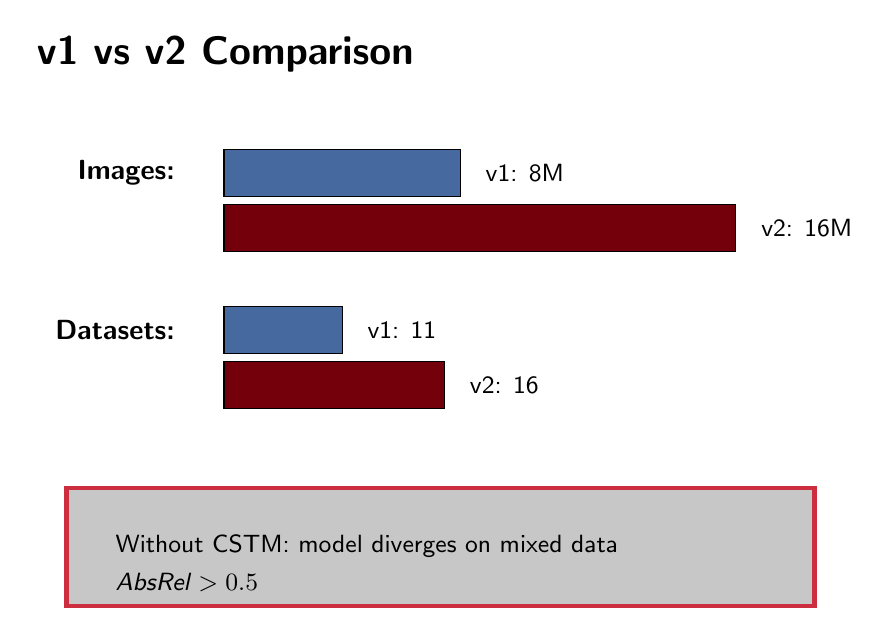
\begin{tikzpicture}[x=1cm, y=1cm]

% Title for comparison
\node[anchor=west, font=\sffamily\bfseries\Large] at (0, 9) {v1 vs v2 Comparison};

% Labels for metrics
\node[anchor=east, font=\sffamily\normalsize\bfseries] at (2, 7.5) {Images:};
\node[anchor=east, font=\sffamily\normalsize\bfseries] at (2, 5.5) {Datasets:};

% v1 Images bar (8M)
\draw[fill=atlantic] (2.5, 7.2) rectangle (5.5, 7.8);
\node[anchor=west, font=\sffamily\small] at (5.7, 7.5) {v1: 8M};

% v2 Images bar (16M)
\draw[fill=garnet] (2.5, 6.5) rectangle (9, 7.1);
\node[anchor=west, font=\sffamily\small] at (9.2, 6.8) {v2: 16M};

% v1 Datasets bar (11)
\draw[fill=atlantic] (2.5, 5.2) rectangle (4, 5.8);
\node[anchor=west, font=\sffamily\small] at (4.2, 5.5) {v1: 11};

% v2 Datasets bar (16)
\draw[fill=garnet] (2.5, 4.5) rectangle (5.3, 5.1);
\node[anchor=west, font=\sffamily\small] at (5.5, 4.8) {v2: 16};

% Callout box for warning
\draw[line width=1.5pt, color=rose, fill=bk30] (0.5, 2) rectangle (10, 3.5);
\node[anchor=west, font=\sffamily\small, text width=8.8cm] at (1, 2.75) {Without CSTM: model diverges on mixed data};
\node[anchor=west, font=\sffamily\small\itshape] at (1, 2.3) {AbsRel $> 0.5$};

\end{tikzpicture}

\end{document}
